\section{3D Graphics}
To define a point in a 3D-space , 3 coordinates are typically used . However in computer graphics \textbf{4} coordinates $x,y,z,w$ called \textbf{homogeneous coordinates} are used :
\begin{itemize}
\item $x,y,z$ are used to define the \textbf{point in the 3D space}
\item $w$ defines a \textbf{scale}, the unit of measure used by the coordinates
\end{itemize}
\begin{figure}[H]
\centering
  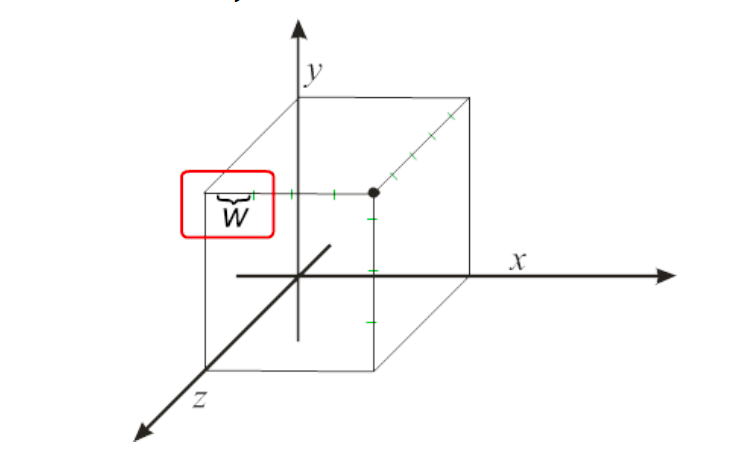
\includegraphics[width=.4\linewidth]{3Dcoor}
\end{figure}
Consequence of using 4 coordinates $\to$  \textbf{infinite} number of coordinates define the same point , in particular all tuples of four values that are \textbf{linearly dependent} represent the same point in 3D space :
$$  (2,2,2.5,0.5),(4,4,5,1) : (4,4,5,1) = 2(2,2,2.5,0.5)$$
The \textbf{real position} of a point in 3D spcae is defined by $w=1$.
To obtain the real position a simple division of \textbf{w} is sufficient.
$$ (x,y,z,w) \to (x',y',z') = (\frac{x}{w}, \frac{y}{w}, \frac{z}{w})$$

\subsection{Affine Transformations}
The process of varying the coordinates of the points  of an object in the space is called \textbf{transformation}.\\
Transformations can be very \textbf{complex} since all points should be repositioned  in a 3D space .\\A large \textbf{set of transformations} with a mathematical concept called \textbf{affine transformations}\\
Objects in 3D space are defined by the coordinates of their points.By applying affine transformations to the coordinates 4 different transformations can be done :
\begin{itemize}
\item \textbf{Translation}
\item \textbf{Scaling}
\item \textbf{Rotation}
\item \textbf{Shear}
\end{itemize}
The new object is drawn using the new points and the corresponding \textbf{primitives}.\\
$$ p=(x,y,z,w) \to p'=(x',y',z',w') $$ 
To express transformations $4x4 $ matrices M can be used. So the new point p' can be obtained by multiplying p by the \textbf{transformation matrix} :
$$ p' = M\cdot p^T $$ or $$ p' = p \cdot M^T $$
depending on the \textbf{convention}

\subsubsection{Translation}
Moves the points of the object while maintaining its \textbf{size \& orientation}.
Translation can be performed along the three axis : $dx,dy,dz$ are the quantities that define how much the object is being moved : 
$$ x' = x+dx $$
$$ y' = y+dy $$
$$ z' = z+dz $$
By using the 4th coordinate the \textbf{translation matrix} can be obtained:

$$ 	\begin{bmatrix}
       1 & 0 & 0 & dx           \\[0.3em]
       0 & 1 & 0 & dy		    \\[0.3em]
       0 & 0 & 1 & dz			\\[0.3em]
       0 & 0 & 0 & 1
     \end{bmatrix} 
	 \cdot
	 \begin{bmatrix}
	  x  \\
	  y	 \\
	  z  \\ 
	  1
	 \end{bmatrix}	
	 =
	 \begin{bmatrix}
	 x+dx \\
	 y+dy \\
	 z+dz \\
	 1
\end{bmatrix}	       
$$
\newpage
\subsubsection{Scaling}
Scaling modifies the \textbf{size of an object} while maintaining constant \textbf{position and orientation}.It can have different effects :
\begin{itemize}
\item \textbf{Enlarge}
\item \textbf{Shrink}
\item \textbf{Deform} ex:Sphere $\to$ rugby ball
\item \textbf{Mirroring} ex: Object on the right $\to$ symmetrical on the left
\end{itemize}
Scale transformations have \textbf{a center} : a point that is \textbf{not moved} during the transformation. The center of transformation can be anywhere on the 3D space ( also outside the object!).\\
Now we assume that the center corresponds to the \textbf{origin}.\\
\begin{itemize}
\item \textbf{Proportional scaling}\\
Enlarges or shrinks the object of the same amount \textbf{s} in all the directions : this leaves the proportions intact.
$$ x' = s \cdot x$$
$$ y' = s \cdot y$$
$$ z' = s \cdot z$$
If $ s > 1 \to $ \textbf{enlarge}\\
Else $ 0< s<1 \to $ \textbf{shrink} 
\item  \textbf{Non proportional scaling}\\
Deforms an object by using different scaling factors $ s_x, s_y,s_z$ that allows shrinking or enlarging in different directions.\\
$$ x' = s_x \cdot x$$
$$ y' = s_y \cdot y$$
$$ z' = s_z \cdot z$$
If $ s_i > 1 \to $ \textbf{enlarge}\\
Else $ 0< s_i<1 \to $ \textbf{shrink}\\
A \textbf{scaling matrix} can be used to represent transformations :
$$	
\begin{bmatrix}
       s_x & 0 & 0 & 0           \\[0.3em]
       0 & s_y & 0 & 0		    \\[0.3em]
       0 & 0 & s_z & 0			\\[0.3em]
       0 & 0 & 0 & 1
     \end{bmatrix} 
$$
\item \textbf{Mirroring}\\
By using \textbf{negative scaling factors} mirroring can be obtained. Three different types exist in 3D space:
\begin{enumerate}
\item \textbf{Planar}\\
Creates a symmetric object with respect to a \textbf{plane} by assigning \textbf{-1} scaling factor to the axis \textbf{perpendicular to the plane}
\begin{figure}[H]
\centering
  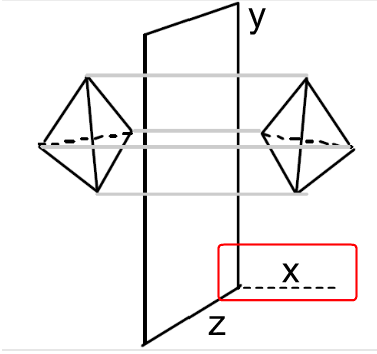
\includegraphics[width=.4\linewidth]{mirroring}
  \caption{$ s_x =-1, s_y=1 ,s_z=1$}
\end{figure}
\newpage
\item \textbf{Axial}\\
Creates a symmetric object with respect to a \textbf{axis} by assigning \textbf{-1} to all scaling factors \textbf{except} the one of the axis.
\begin{figure}[H]
\centering
  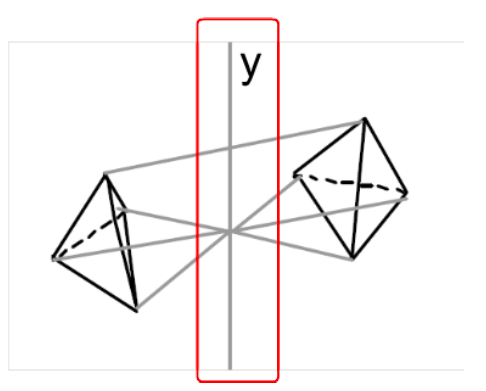
\includegraphics[width=.4\linewidth]{mirroring2}
  \caption{$ s_x =-1, s_y=1 ,s_z=-1$}
\end{figure}
\item \textbf{Central}\\
Creates a symmetric object with respect to the \textbf{origin}.It is obtained by assigning \textbf{-1} to all scaling factors.
\begin{figure}[H]
\centering
  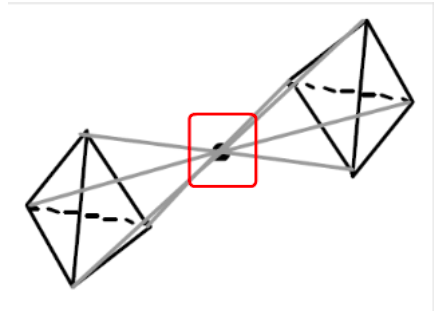
\includegraphics[width=.4\linewidth]{mirroring3}
  \caption{$ s_x =-1, s_y=-1 ,s_z=-1$}
\end{figure}
\end{enumerate}
Notice that if a scaling factor of \textbf{0} is chosen it \textbf{flattens} the image along that axis. This makes the transformation matrix \textbf{not invertible}
\end{itemize}

\subsubsection{Rotation}
Varies the objects \textbf{orientation} leaving unchanged its \textbf{position and size}. Rotation happens along a chosen axis , a line where points are \textbf{unaffected} by the transformation.\\
Rotation can occur also on non conventional axis but we will mainly consider rotations along x,y,z axis passing through the origin.\\
A rotation of angle $\alpha$ about the z-axis :
$$ x' = x \cdot cos\alpha - y \cdot sin\alpha$$
$$ y' = x \cdot sin\alpha + y \cdot cos\alpha$$
$$ z' = z$$
As the z-axis is the \textbf{axis of rotation} its points remain unchanged.
A rotation of angle $\alpha$ about the y-axis :
$$ x' = x \cdot cos\alpha + z \cdot sin\alpha$$
$$ y' = y $$
$$ z' = -x \cdot sen\alpha + z \cdot cos\alpha$$
A rotation of angle $\alpha$ about the x-axis :
$$ x' = x$$
$$ y' = y \cdot cos\alpha -z \cdot sin\alpha$$
$$ z' = y \cdot sin\alpha +z \cdot cos\alpha$$

\begin{figure}[H]
\centering
  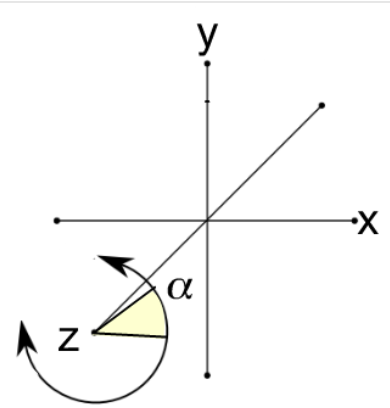
\includegraphics[width=.4\linewidth]{rotation}
  \caption{Z-Axis rotation}
 \end{figure}
 
Again matrices can be used to express rotation :\\ \hfill
$	
R_z= \begin{bmatrix}
       cos\alpha & -sin\alpha & 0 & 0        \\[0.1em]
       sin\alpha & cos\alpha & 0 & 0		    \\[0.1em]
       0 & 0 & 1 & 0							\\[0.1em]
       0 & 0 & 0 & 1
     \end{bmatrix} 
$ $     
R_y= \begin{bmatrix}
       cos\alpha & 0 & sin\alpha & 0         \\[0.1em]
       0 & 1 & 0 & 0		    				    \\[0.1em]
       -sin\alpha & 0 & cos\alpha & 0	    \\[0.1em]
       0 & 0 & 0 & 1
     \end{bmatrix}
$ $    
R_x= \begin{bmatrix}
       1 & 0 & 0 & 0          			    \\[0.1em]
       0 & cos\alpha & -sin\alpha & 0		\\[0.1em]
       0 & sin\alpha & cos\alpha & 0			\\[0.1em]
       0 & 0 & 0 & 1
     \end{bmatrix}  
$
\newpage
\subsection{Shear}
Shear bends the objects in one direction. It has an \textbf{axis} and \textbf{center}.
Considering axis y and the origin as center
\begin{figure}[H]
\centering
  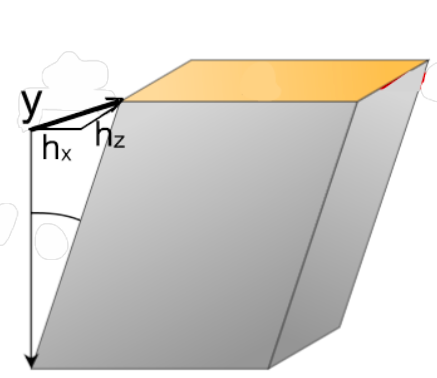
\includegraphics[width=.4\linewidth]{shear}
 \end{figure}
as the values of y increase the object is bent following the direction of a vector defined by two values ( $h_x,h_z$ in this case ) :
$$ x'= x+y\cdot h_x$$
$$ y'=y$$
$$ z'= z+y\cdot h_z$$
Along the \textbf{x-axis}:
$$ x'= x$$
$$ y'=y+x \cdot h_y$$
$$ z'= z+x\cdot h_z$$
Along the \textbf{z-axis}:
$$ x'= x+z \cdot h_x$$
$$ y'=y+z \cdot h_y$$
$$ z'= z$$
Again matrices can be used to express shear :\\ \hfill
$	
H_x(h_y,h_z)= \begin{bmatrix}
       1 & 0 & 0 & 0        \\[0.1em]
       h_y & 1 & 0 & 0		    \\[0.1em]
       h_z & 0 & 1 & 0							\\[0.1em]
       0 & 0 & 0 & 1
     \end{bmatrix} 
$ $     
H_y(h_x,h_z)= \begin{bmatrix}
       1 & h_x & 0 & 0         \\[0.1em]
       0 & 1 & 0 & 0		    				    \\[0.1em]
       0 & h_z & 0 & 0	    \\[0.1em]
       0 & 0 & 0 & 1
     \end{bmatrix}
$ $    
H_z(h_x,h_y)= \begin{bmatrix}
       1 & 0 & h_x & 0          			    \\[0.1em]
       0 & 1 & h_y & 0		\\[0.1em]
       0 & 0 & 1 & 0			\\[0.1em]
       0 & 0 & 0 & 1
     \end{bmatrix}  
$